\newpage

\section{Results and discussion}
\label{Sec:Results}

In this section, the results of the \pT-dependent non-linear flow modes $v_{4,22}$, $v_{5,32}$, $v_{6,33}$ and $v_{6,222}$ of identified particles are presented for various centrality intervals in Pb--Pb collisions at \sNN. We first present the centrality and \pT~dependence of $v_{\rm n,mk}$ in Sec. \ref{SubSec:pTdependence}. The scaling properties of the non-linear flow modes are also discussed in this section. These results are compared with $v_{\rm n}$ measurements for the same particle species in Sec. \ref{SubSec:comparewithvn}. Finally, the comparison with two model calculations is shown in Sec. \ref{SubSec:hydro}. Note that in some of the following sections the same data are used in different representations to highlight the various physics implications of the measurements in each section.

\subsection{Centrality and \pT~dependence of non-linear flow modes}
\label{SubSec:pTdependence}

Figure \ref{v422_centralityDependence} presents the magnitude of the non-linear mode for the fourth order flow coefficient, $v_{4,22}(p_{\rm{T}})$, for \pion, \kaon, \Ks, \proton, \lambdas~and the $\phi$-meson in a wide range of centrality intervals, i.e.\,0--5\% up to 50--60\%. For the $\phi$-meson, the results are reported from the 10--20\% up to the 40--50\% centrality interval, where $v_{4,22}$ can be measured accurately. The magnitude of this non-linear flow mode rises steeply with increasing centrality interval from 0--5\% to 40--50\% for all particle species. This increase is expected as $v_{4,22}$ reflects the contribution of the second order eccentricity, $\varepsilon_{2}$, which increases from central to peripheral collisions, in $v_{4}$ \cite{Alver:2010gr, Acharya:2017zfg}. For more peripheral collisions (i.e. 50--60\%), the magnitude of $v_{4,22}$ does not increase further with respect to the neighbouring centrality interval (40--50\%). This effect that was observed also in $v_n$ measurements \cite{Abelev:2014pua,Acharya:2018zuq} is probably due to the shorter lifetime of the produced system in more peripheral collisions, which prevents $v_{4,22}$ from developing further. 


\begin{figure}[!htb]
\begin{center}
\includegraphics[scale=0.82]{figures/results/All_v422_gap00_CentDep_PID2.pdf}
\end{center}
\caption{The \pT-differential $v_{4,22}$ for different centrality intervals of Pb--Pb collisions at \sNN~grouped by particle species. Statistical and systematic uncertainties are shown as bars and boxes, respectively.}
\label{v422_centralityDependence}
\end{figure}
 
Figure \ref{v523_centralityDependence} presents the non-linear mode for the fifth order flow coefficient, i.e. $v_{5,32}(p_{\rm{T}})$, of \pion, \kaon, \Ks, \proton, and \lambdas~for the same range of centrality intervals, i.e. 0--5\% up to 50--60\%. Statistical precision limits extending the measurements of non-linear flow modes of the $\phi$-meson for ${\rm n}>4$. The measurements show a significant increase in the magnitude of this non-linear flow mode with increasing centrality percentile. This is due to the fact that $v_{5,32}(p_{\rm{T}})$ has a contribution from both $\varepsilon_{2}$ and $\varepsilon_{3}$. It is shown in MC studies that $\varepsilon_{2}$ and to a smaller extent, $\varepsilon_{3}$ increase for peripheral collisions \cite{Alver:2010gr}. 

\begin{figure}[!htb]
\begin{center}
\includegraphics[scale=0.82]{figures/results/All_v523_gap00_CentDep_PID2.pdf}
\end{center}
\caption{The \pT-differential $v_{5,32}$ for different centrality intervals of Pb--Pb collisions at \sNN~grouped by particle species. Statistical and systematic uncertainties are shown as bars and boxes, respectively.}
\label{v523_centralityDependence}
\end{figure}

Figures \ref{v633_centralityDependence} and \ref{v6222_centralityDependence} present the non-linear terms for the sixth order flow coefficient, i.e. $v_{6,33}(p_{\rm{T}})$ for \pion, \kaon, \Ks, \proton~and \lambdas~for the 0--5\% up to 40--50\% centrality intervals and $v_{6,222}(p_{\rm{T}})$ for \pion, \kaon, \proton~for the 0--5\% up to 50--60\% centrality intervals. As expected, measurements of $v_{6,222}(p_{\rm{T}})$ which probe the contribution of $\varepsilon_2$, show an increase in the magnitude of this non-linear flow mode with increasing centrality percentile. On the other hand, the $v_{6,33}(p_{\rm{T}})$ measurements, which probe the contribution of $\varepsilon_3$, present little to no dependence on centrality as previously observed for charged particles in \cite{Acharya:2017zfg}. 

\begin{figure}[!htb]
\begin{center}
\includegraphics[scale=0.82]{figures/results/All_v633_gap00_CentDep_PID2.pdf}
\end{center}
\caption{The \pT-differential $v_{6,33}$ for different centrality intervals of Pb--Pb collisions at \sNN~grouped by particle species. Statistical and systematic uncertainties are shown as bars and boxes, respectively.}
\label{v633_centralityDependence}
\end{figure}

\begin{figure}[!htb]
\begin{center}
\includegraphics[scale=0.82]{figures/results/All_v6222_gap00_CentDep_PID2.pdf}
\end{center}
\caption{The \pT-differential $v_{6,222}$ for different centrality intervals of Pb--Pb collisions at \sNN~grouped by particle species. Statistical and systematic uncertainties are shown as bars and boxes, respectively.}
\label{v6222_centralityDependence}
\end{figure}

\newpage

In Fig. \ref{v422_particleDependence} the same data points are grouped by centrality interval to highlight how $v_{4,22}$ develops for a given centrality for various particle species as a function of \pT.
A clear mass ordering can be seen in the low \pT~region (i.e. \pT $< 2.5$ \GeV) for all collision centralities. This mass ordering arises from the interplay between radial flow and the initial spatial anisotropy, generated from both the geometry and the fluctuating initial energy density profile. This creates a depletion in the particle spectra at lower \pT~values which becomes larger in-plane than out-of plane due to the velocity profile. This naturally leads to lower $v_{4,22}$(\pT) values for heavier particles \cite{Voloshin:1996nv, Huovinen:2001cy, Shen:2011eg}. Similarly, Figs. \ref{v523_particleDependence}, \ref{v633_particleDependence} and \ref{v6222_particleDependence} show the \pT-differential $v_{5,32}$, $v_{6,33}$ and $v_{6,222}$, respectively, of different particle species for each centrality interval. A clear mass ordering is seen in the low \pT~region, (i.e. \pT $< 2.5$ \GeV), for $v_{5,32}(p_{\rm{T}})$ and to a smaller extent for $v_{6,33}(p_{\rm{T}})$ as well as for some centrality intervals of $v_{6,222}(p_{\rm{T}})$.

\begin{figure}[!htb]
\begin{center}
\includegraphics[scale=0.82]{figures/results/All_v422_gap00_PID2_3by3.pdf}
\end{center}
\caption{The \pT-differential $v_{4,22}$ for different particle species grouped into different centrality intervals of Pb--Pb collisions at \sNN. Statistical and systematic uncertainties are shown as bars and boxes, respectively.}
\label{v422_particleDependence}
\end{figure}

\begin{figure}[!htb]
\begin{center}
\includegraphics[scale=0.82]{figures/results/All_v523_gap00_PID2_3by3.pdf}
\end{center}
\caption{The \pT-differential $v_{5,32}$ for different particle species grouped into different centrality intervals of Pb--Pb collisions at \sNN. Statistical and systematic uncertainties are shown as bars and boxes, respectively.}
\label{v523_particleDependence}
\end{figure}

\begin{figure}[!htb]
\begin{center}
\includegraphics[scale=0.82]{figures/results/All_v633_gap00_PID2_3by2.pdf}

\end{center}
\caption{The \pT-differential $v_{6,33}$ for different particle species grouped into different centrality intervals of Pb--Pb collisions at \sNN. Statistical and systematic uncertainties are shown as bars and boxes, respectively.}
\label{v633_particleDependence}
\end{figure}

\begin{figure}[!htb]
\begin{center}
\includegraphics[scale=0.82]{figures/results/All_v6222_gap00_PID2_3by3.pdf}

\end{center}
\caption{The \pT-differential $v_{6,222}$ for different particle species grouped into different centrality intervals of Pb--Pb collisions at \sNN. Statistical and systematic uncertainties are shown as bars and boxes, respectively.}
\label{v6222_particleDependence}
\end{figure}

\newpage

In addition, in the intermediate \pT~region (for \pT $> 2.5$ \GeV) the data points of Figs. \ref{v422_particleDependence}-\ref{v6222_particleDependence} exhibit a particle type grouping. In particular, the data points form two groups, one for mesons and one for baryons with the values of $v_{n,mk}$ of the latter being larger. This particle type grouping was previously observed in $v_{n}$ measurements of various particle species \cite{Abelev:2014pua,Adam:2016nfo,Acharya:2018zuq,Adams:2003am,Abelev:2007qg,Adler:2003kt,Adare:2006ti}. 
This grouping was explained in Ref. \cite{Molnar:2003ff} in the picture of particle production via quark coalescence indicating that flow develops at the partonic stage. In this picture, known as NCQ scaling, the flow of mesons (baryons) is roughly twice (thrice) the flow of their constituent quarks in the intermediate transverse momentum region \cite{Voloshin:2002wa,Molnar:2003ff}. The ALICE measurements show that this scaling at the LHC energies holds at an approximate level of 20\% for $v_{n}$ \cite{Abelev:2014pua,Adam:2016nfo,Acharya:2018zuq}. 

Figures \ref{v422_NCQ}, \ref{v523_NCQ}, \ref{v633_NCQ} and \ref{v6222_NCQ} present $v_{4,22}$, $v_{5,32}$, $v_{6,33}$ and $v_{6,222}$, respectively, scaled by the number of constituent quarks ($n_{q}$) as a function of \pTnq~for \pion, \kaon, \Ks, \proton, \lambdas~and the $\phi$-meson grouped in different centrality intervals. The scaling is consistent with the observations reported for higher order anisotropic flow coefficients \cite{Acharya:2018zuq}. It is seen that for the non-linear flow modes this scaling holds at an approximate level ($\pm$20\%) for \pT $> 1$ \GeVc,~where quark coalescence is expected to be the dominant process.

\begin{figure}[!htb]
\begin{center}
\includegraphics[scale=0.82]{figures/scaling/All_v422_gap00_NCQ_3by3.pdf}
\end{center}
\caption{The $p_{\rm{T}}/n_{q}$-dependence of $v_{4,22}/n_{q}$ for different particle species grouped into different centrality intervals of Pb--Pb collisions at \sNN. Statistical and systematic uncertainties are shown as bars and boxes, respectively.}
\label{v422_NCQ}
\end{figure}

\begin{figure}[!htb]
\begin{center}
\includegraphics[scale=0.82]{figures/scaling/All_v523_gap00_NCQ_3by3.pdf}
\end{center}
\caption{The $p_{\rm{T}}/n_{q}$-dependence of $v_{5,32}/n_{q}$ for different particle species grouped into different centrality intervals of Pb--Pb collisions at \sNN. Statistical and systematic uncertainties are shown as bars and boxes, respectively.}
\label{v523_NCQ}
\end{figure}

\begin{figure}[!htb]
\begin{center}
\includegraphics[scale=0.82]{figures/scaling/All_v633_gap00_NCQ_3by2.pdf}
\end{center}
\caption{The $p_{\rm{T}}/n_{q}$-dependence of $v_{6,33}/n_{q}$ for different particle species grouped into different centrality intervals of Pb--Pb collisions at \sNN. Statistical and systematic uncertainties are shown as bars and boxes, respectively.}
\label{v633_NCQ}
\end{figure}

\begin{figure}[!htb]
\begin{center}
\includegraphics[scale=0.82]{figures/scaling/All_v6222_gap00_NCQ_3by3.pdf}
\end{center}
\caption{The $p_{\rm{T}}/n_{q}$-dependence of $v_{6,222}/n_{q}$ for different particle species grouped into different centrality intervals of Pb--Pb collisions at \sNN. Statistical and systematic uncertainties are shown as bars and boxes, respectively.}
\label{v6222_NCQ}
\end{figure}


\subsection{Comparison with $v_{\rm n}$ of identified particles}
\label{SubSec:comparewithvn}

The comparison of the features discussed before i.e. mass ordering and particle type grouping between the non-linear and the anisotropic flow coefficient is of particular interest.  Based on a naive expectation the mass ordering should develop quantitatively in a different way between the non-linear (i.e. due to the dependence on $\varepsilon_{2}^{2}$) and the anisotropic flow coefficient. In parallel, if coalescence is the dominant particle production mechanism in the intermediate \pT~region, one expects a similar grouping between $v_{\rm n}^{\rm NL}$ and $v_{\rm n}$. Such a comparison could only be performed for $v_{4,22}$(\pT) (this study) and the $v_{4}$(\pT) measurements \cite{Acharya:2018zuq} and was done by taking the difference between pions and protons at a given \pT~in both modes and normalising it by the integrated flow of the corresponding mode for charged particles \cite{Adam:2016izf} ($[v_{4}^{\pi^{\pm}} -  v_{4}^{\rm p+\bar{p}}](p_{\rm T}) / v_{4}^{\rm h^{\pm}}$). This comparison is shown in Fig. \ref{massOrderingComparison} for the 0--5\% up to the 40--50\% centrality interval. It can be seen that in the low \pT~region (\pT~< $2.5-3$ \GeV) where the mass ordering is prominent, the data points exhibit a general agreement for all centrality intervals. However, there is a hint that the relative ratio for $v_{4,22}$ is smaller than the one of the $v_{4}$ for \pT~$< 0.8$ \GeV~and for the centrality intervals 0--30\%.
 If this difference and its centrality dependence persist for low values of \pT, it could indicate that the hydrodynamic evolution is reflected differently in $v_{4}$ and $v_{4,22}$ and could be explained by the contribution of $\varepsilon_{2}^{2}$.  As stated earlier, the mass splitting is a result of an interplay of radial and anisotropic flow, leading to a stronger in-plane expansion compared to out-of-plane, and the particle thermal motion. Particles with larger mass have smaller thermal velocities, and are thus affected stronger by the difference between in- and out-of-plane expansion velocities, thus leading to the mass splitting of $v_{n}$(\pT). The comparison of the \pT~dependence of $v_{n}^{\rm NL}$ and $v_{n}$ can therefore provide a unique opportunity to test this picture, as it would allow results for the cases of exactly the same average radial flow and temperature, but differing in anisotropic flow to be compared. On the other hand, in the intermediate \pT~region (\pT~> 2.5 \GeV), the same comparison shows that the results are compatible in all centrality intervals within one standard deviation. This implies a similar particle type grouping between $v_{4}$ and $v_{4,22}$ which is in line with the expectation that quark coalescence affects both flow modes  similarly.

\begin{figure}[!htb]
\begin{center}
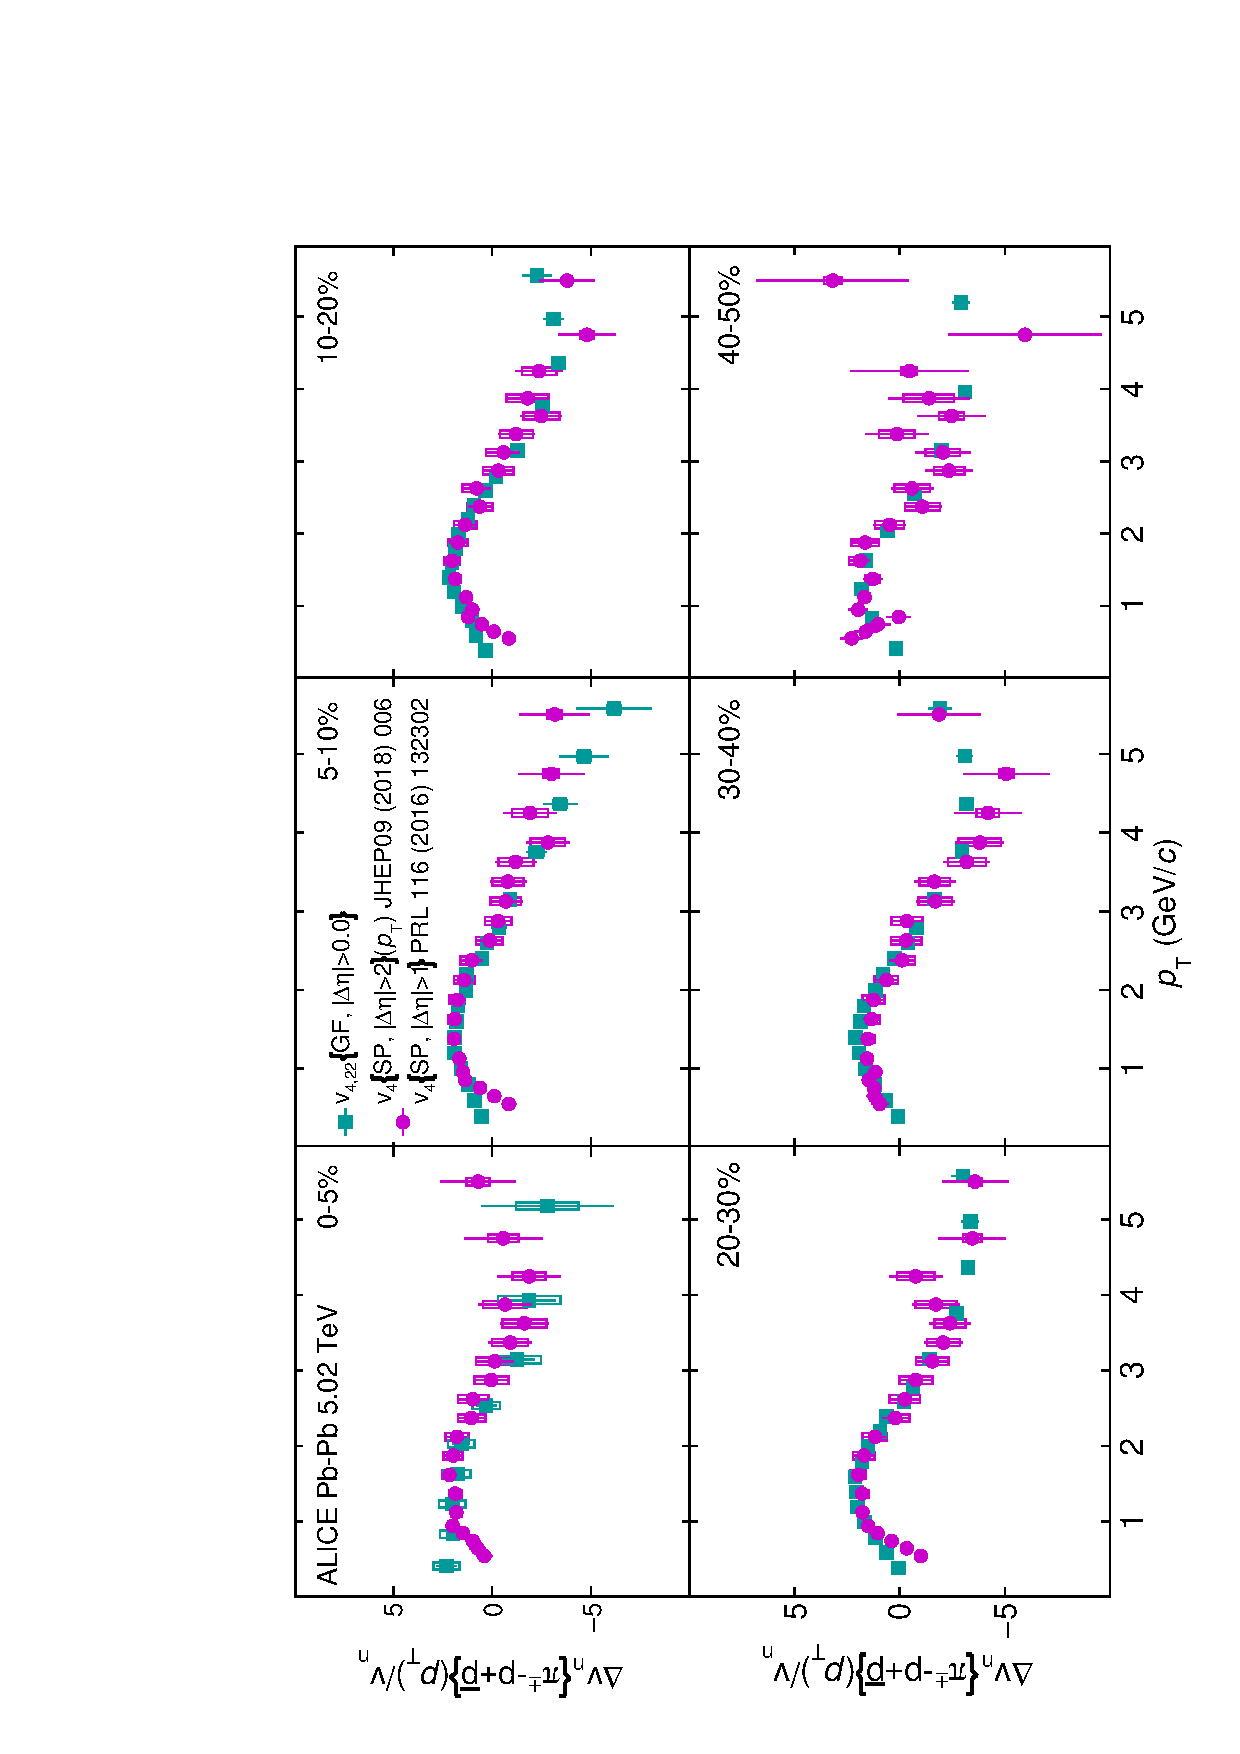
\includegraphics[scale=0.6]{figures/results/massOrdering_vn_pion_proton_to_charged.pdf}
\end{center}
\caption{The comparison between $[v_{4,22}^{\pi^{\pm}} -  v_{4,22}^{\rm p+\bar{p}}](p_{\rm T}) / v_{4,22}^{\rm h^{\pm}} $ and $[v_{4}^{\pi^{\pm}} -  v_{4}^{\rm p+\bar{p}}](p_{\rm T}) / v_{4}^{\rm h^{\pm}} $  grouped into different centrality intervals of Pb--Pb collisions at \sNN. Statistical and systematic uncertainties are shown as bars and boxes, respectively.}
\label{massOrderingComparison}
\end{figure}

\newpage
\subsection{Comparison with models}
\label{SubSec:hydro}

The comparison of various anisotropic flow measurements and hydrodynamic calculations are presented and discussed in great detail in \cite{Xu:2016hmp, McDonald:2016vlt, Zhao:2017yhj}. A recent comparison between $v_{n}$ measurements reported by the ALICE collaboration \cite{Acharya:2018zuq} and two hydrodynamic calculations from \cite{Zhao:2017yhj} shed new light on the initial conditions and the transport properties of the created system in Pb--Pb collisions. Both hydrodynamic calculations are based on iEBE-VISHNU \cite{Shen:2014vra}, an event-by-event version of the VISHNU hybrid model \cite{Song:2010aq} coupling $2+1$~dimensional viscous hydrodynamics (VISH2+1) \cite{Song:2007fn} to a hadronic cascade model (UrQMD). The initial conditions used for these calculations are described by AMPT \cite{Lin:2004en} and \trento~ \cite{Moreland:2014oya}, both with $\tau_{0}$=0.6 fm/$c$ and $T_{sw}$ =148 MeV \cite{Bernhard:2016tnd}. For AMPT initial conditions, constant values of specific shear viscosity over entropy density ($\eta/s =0.08$, the lower limit conjectured by AdS/CFT) and bulk viscosity over entropy density ($\zeta/s = 0$) are utilised. The version of the model that uses \trento~ \cite{Moreland:2014oya} initial conditions incorporates temperature dependent specific shear and bulk viscosities extracted from the global bayesian analysis \cite{Bernhard:2016tnd}. \footnote{ For simplicity in the rest of this article the model with AMPT initial conditions, $\eta/s =0.08$ and $\zeta/s =0$ is referred to as AMPT and the model with \trento~initial conditions, $\eta/s(\rm{T})$ and $\zeta/s(\rm{T})$ is referred to as \trento.} 

The comparison between $v_{n}$ measurements and these two hydrodynamic calculations illustrates a qualitative agreement. This agreement between the data and the models depends on the particle species, transverse momentum range and centrality percentile. Overall, the AMPT model reproduces the measurements more accurately than the \trento~model \cite{Acharya:2018zuq}. In order to further investigate the performance of these two models in reproducing the $v_{\rm n}$ measurements, and provide a quantitative comparison, the relative ratios between each model and the measurements of \pion, \kaon~and \proton~are obtained. Table \ref{ModelDataComparisonflow} summarises these relative ratios. The values represent the ranges across all centralities that each model is able to describe the measurements of $v_n$ for each particle species. Comparisons between the performance of the two models show that the AMPT calculations reproduce $v_{2}$ slightly better that \trento. Both models reproduce the $v_{3}$ measurements relatively better than the $v_{2}$, however AMPT performs better than \trento. Finally, the comparison between the models and the $v_{4}$ measurements show that AMPT has an absolute better performance compared to \trento. These values should be taken with caution as $v_{4}$ has larger uncertainties with respect to $v_{3}$ and $v_{2}$. 

\begin{table}[!h]
\centering
\caption{List of minimum and maximum values of the fit with a constant function to relative ratios between data and each model for  $v_{\rm n} ({\rm n}=2,3,4)$ of \pion, \kaon~and \proton. The percentages show deviations of the fit from unity obtained for the 0--5\% up to 40--50\% centrality intervals.}
\resizebox{0.81\textwidth}{!}{\begin{tabular}{ |p{4.5cm} |l|c|c|c|c|c|c|c|c|c|}
\hline
\multicolumn{1}{| c |}{} & \multicolumn{3}{| c |}{ $v_{2}$ } & \multicolumn{3}{| c |}{ $v_{3}$} & \multicolumn{3}{| c |}{ $v_{4}$}  \\
\hline
Model  & \pion &  \kaon & \proton &  \pion & \kaon & \proton &  \pion &  \kaon & \proton \\ \hline  \hline
AMPT calculations & 3--13\% & 0--16\% & 0--20\% & 0--8\% & 5--12\% & 0--4\%& 6--12\% & 5--12\% & 0--4\%  \\
\trento~ calculations & 6--17\% & 0--19\% & 3--19\% & 2--15\% & 7--22\% & 0--11\% & 7--25\% & 16--28\% & 0--21\% \\
 \hline
\end{tabular}}
\label{ModelDataComparisonflow}
\end{table}

\begin{table}[!h]
\caption{List of minimum and maximum values of the fit with a constant function to relative ratios between the data and each model for  $v_{\rm n,mk}$ of \pion, \kaon~and \proton. The percentages show deviations of the fit from unity obtained for the 0--10\% up to 50--60\% (40--50\% for $v_{6,33}$) centrality intervals.}
\resizebox{\textwidth}{!}{\begin{tabular}{ |p{4.5cm} |l|c|c|c|c|c|c|c|c|c|c|c|c|}
\hline
\multicolumn{1}{| c |}{} & \multicolumn{3}{| c |}{ $v_{4,22}$ } & \multicolumn{3}{| c |}{ $v_{5,32}$} & \multicolumn{3}{| c |}{ $v_{6,33}$} & \multicolumn{3}{| c |}{ $v_{6,222}$} \\
\hline
Model  & \pion &  \kaon & \proton &  \pion & \kaon & \proton &  \pion &  \kaon & \proton &  \pion &  \kaon & \proton \\ \hline  \hline
AMPT calculations &  5--32\% & 2--30\%  & 3--30\% & 3--28\%  & 5--29\% &  1--65\% & 0--46\% & 0--46\% & 0--97\% & 6--52\% & 0--80\%  & 0--118\% \\
\trento~ calculations & 0--30\% & 4--33\% & 0--21\% &  24--49\% & 33--97\% & 12--58\% & 0--43\% & 0--46\% & 0--95\% & 0--20\% & 0--34\% & 0--78\%\\
 \hline
\end{tabular}}
\label{ModelDataComparisonNLflow}
\end{table}

To achieve additional constraints on the initial conditions and transport properties of the system and test the validity of these hydrodynamic models, a comparison is performed between the measured \pT-dependent non-linear flow modes for \pion, \kaon, \proton, \Ks~and \lambdas~with the same two hydrodynamical calculations reported in \cite{Zhao:2017yhj}. Figures \ref{v422_model}--\ref{v6222_model} present the comparison between the measurements and the two model predictions for the \pT-differential $v_{4,22}$, $v_{5,32}$, $v_{6,33}$ and $v_{6,222}$, respectively, for \pion, \kaon~and \proton~and Figs. \ref{v422_model_KL}--\ref{v633_model_KL} present these comparisons for the \pT-differential $v_{4,22}$, $v_{5,32}$ and $v_{6,33}$ for \Ks~and \lambdas~for the 0--10\% up to 50--60\% centrality interval (40--50\% centrality interval for $v_{6,33}$) of Pb--Pb collisions at \sNN. The solid bands show the AMPT model and the hatched bands represent the \trento~ calculations. The bottom panels in each plot in Figs. \ref{v422_model}--\ref{v633_model_KL} show the difference between the models and the measurement. Both \trento~and AMPT reproduce the mass ordering feature at $p_{\rm{T}}<2.5$ \GeV~for all non-linear flow modes. In particular, the comparison between the models and the measurements of $v_{4,22}$ reveals that \trento~reproduces the data very well from the 0--10\% up to 30--40\% centrality interval and fails to reproduce the measurements for the remaining more peripheral centrality intervals. On the other hand, AMPT overestimates the measurements from the 0--10\% up to 30--40\% centrality interval. For the 40--50\% centrality interval, it reproduces the measurements for all particle species except \pion, where it slightly underestimates the results. For more peripheral collisions, it reproduces the \kaon, \proton~and \lambdas~measurements and underestimates the results for \pion~and \Ks. 

In a similar attempt to the comparison between the $v_{n}$ measurement and the model calculation in Tab. \ref{ModelDataComparisonflow}, the performance of these models were further studied for $v_{n,mk}$ by taking the relative ratios between each model and the measurements of \pion, \kaon~and \proton. These relative ratios are summarised in Tab. \ref{ModelDataComparisonNLflow} where \trento~ calculations reproduce $v_{4,22}$ better than AMPT by $\sim$7\%. Comparisons between Tab. \ref{ModelDataComparisonNLflow} and \ref{ModelDataComparisonflow} show that the AMPT calculations reproduce $v_{4,22}$ with $\sim$20\% higher discrepancy on average compared to $v_{4}$, and, the \trento~calculations perform equally well for $v_{4,22}$ as for $v_{4}$. It is necessary to stress, however, that the non-linear flow modes have smaller magnitudes with respect to $v_{n}$ and any discrepancy between the models and the data becomes magnified in the ratios reported in Tab. \ref{ModelDataComparisonNLflow}. 

For $v_{5,32}$, the comparison is different, with the \trento~ predictions overestimating the measurements for all centrality intervals, and AMPT reproducing the data better than \trento. The AMPT model overestimates the measurements from the 0--10\% to 20--30\% centrality interval. It underestimates the measurements of \pion, \kaon~and \proton~for more peripheral collisions while it reproduces the measurements of \Ks~and \lambdas~relatively well up to the 40--50\% centrality interval. These comparisons are reflected in Tab. \ref{ModelDataComparisonNLflow} where AMPT performs on average 20--27\% better than \trento~for \pion, \kaon~and \proton. 

For $v_{6,33}$, both models reproduce the data for the 0--10\% centrality interval. For the 10--20\% up to 30--40\% centrality interval, AMPT reproduces the data while \trento~overestimates the measurements. Finally, the comparison with $v_{6,222}$ shows an agreement between both models and the measurements of \pion, \kaon~and \proton~at 0--10\% up to 30--40\% centrality intervals  \footnote{The ratios reported for $v_{6,33}$ and $v_{6,222}$ in Tab. \ref{ModelDataComparisonNLflow} are not to be taken at face value as the magnitudes of these two non-linear flow modes are almost zero.}. 


 \begin{figure}[h]
\begin{center}
\includegraphics[scale=0.73]{figures/model/TrentoAndAMPT_v422_gap00_PID2.pdf}
\end{center}
\caption{The \pT-differential $v_{4,22}$ of \pion, \kaon~and \proton~in the 0--10\% up to 50--60\% centrality intervals of Pb--Pb collisions at \sNN compared with iEBE-VISHNU hybrid models with two different sets of initial parameters: AMPT initial conditions ($\eta/s$= 0.08 and $\zeta/s$ = 0) shown as solid bands and \trento~initial conditions ($\eta/s({\rm T})$ and $\zeta/s({\rm T})$) as hatched bands. The bottom panels show the difference between the measurements and each model. Statistical and systematic uncertainties are shown as bars and boxes, respectively.}
\label{v422_model}
\end{figure}

\begin{figure}[h]
\begin{center}
\includegraphics[scale=0.73]{figures/model/TrentoAndAMPT_v523_gap00_PID2.pdf}
\end{center}
\caption{The \pT-differential $v_{5,32}$ of \pion, \kaon~and \proton~in the 0--10\% up to 50--60\% centrality intervals of Pb--Pb collisions at \sNN compared with iEBE-VISHNU hybrid models with two different sets of initial parameters: AMPT initial conditions ($\eta/s$= 0.08 and $\zeta/s$ = 0) shown as solid bands and \trento~initial conditions ($\eta/s({\rm T})$ and $\zeta/s({\rm T})$) as hatched bands. The bottom panels show the difference between the measurements and each model. Statistical and systematic uncertainties are shown as bars and boxes, respectively.}
\label{v523_model}
\end{figure}


\begin{figure}[h]
\begin{center}
\includegraphics[scale=0.73]{figures/model/TrentoAndAMPT_v633_gap00_PID2.pdf}
\end{center}
\caption{The \pT-differential $v_{6,33}$ of \pion, \kaon~and \proton~in the 0--10\% up to 40--50\% centrality intervals of Pb--Pb collisions at \sNN compared with iEBE-VISHNU hybrid models with two different sets of initial parameters: AMPT initial conditions ($\eta/s$= 0.08 and $\zeta/s$ = 0) shown as solid bands and \trento~initial conditions ($\eta/s({\rm T})$ and $\zeta/s({\rm T})$) as hatched bands. The bottom panels show the difference between the measurements and each model. Statistical and systematic uncertainties are shown as bars and boxes, respectively.}
\label{v633_model}
\end{figure}

\begin{figure}[h]
\begin{center}
\includegraphics[scale=0.73]{figures/model/TrentoAndAMPT_v6222_gap00_PID2.pdf}
\end{center}
\caption{The \pT-differential $v_{6,222}$ of \pion, \kaon~and \proton~in the 0--10\% up to 50--60\% centrality intervals of Pb--Pb collisions at \sNN compared with iEBE-VISHNU hybrid models with two different sets of initial parameters: AMPT initial conditions ($\eta/s$= 0.08 and $\zeta/s$ = 0) shown as solid bands and \trento~initial conditions ($\eta/s({\rm T})$ and $\zeta/s({\rm T})$) as hatched bands. The bottom panels show the difference between the measurements and each model. Statistical and systematic uncertainties are shown as bars and boxes, respectively.}
\label{v6222_model}
\end{figure}



 \begin{figure}[h]
\begin{center}
\includegraphics[scale=0.73]{figures/model/TrentoAndAMPT_v422_gap00_LambdaK0s.pdf}
\end{center}
\caption{The \pT-differential $v_{4,22}$ of \Ks~and \lambdas~in the 0--10\% up to 50--60\% centrality intervals of Pb--Pb collisions at \sNN compared with iEBE-VISHNU hybrid models with two different sets of initial parameters: AMPT initial conditions ($\eta/s$= 0.08 and $\zeta/s$ = 0) shown as solid bands and \trento~initial conditions ($\eta/s({\rm T})$ and $\zeta/s({\rm T})$) as hatched bands. The bottom panels show the difference between the measurements and each model. Statistical and systematic uncertainties are shown as bars and boxes, respectively.}
\label{v422_model_KL}
\end{figure}


 \begin{figure}[h]
\begin{center}
\includegraphics[scale=0.73]{figures/model/TrentoAndAMPT_v523_gap00_LambdaK0s.pdf}
\end{center}
\caption{The \pT-differential $v_{5,32}$ of \Ks~and \lambdas~in the 0--10\% up to 50--60\% centrality intervals of Pb--Pb collisions at \sNN compared with iEBE-VISHNU hybrid models with two different sets of initial parameters: AMPT initial conditions ($\eta/s$= 0.08 and $\zeta/s$ = 0) shown as solid bands and \trento~initial conditions ($\eta/s({\rm T})$ and $\zeta/s({\rm T})$) as hatched bands. The bottom panels show the difference between the measurements and each model. Statistical and systematic uncertainties are shown as bars and boxes, respectively.}
\label{v523_model_KL}
\end{figure}


 \begin{figure}[h]
\begin{center}
\includegraphics[scale=0.73]{figures/model/TrentoAndAMPT_v633_gap00_LambdaK0s.pdf}
\end{center}
\caption{The \pT-differential $v_{6,33}$ of \Ks~and \lambdas~in the 0--10\% up to 40--50\% centrality intervals of Pb--Pb collisions at \sNN compared with iEBE-VISHNU hybrid models with two different sets of initial parameters: AMPT initial conditions ($\eta/s$= 0.08 and $\zeta/s$ = 0) shown as solid bands and \trento~initial conditions ($\eta/s({\rm T})$ and $\zeta/s({\rm T})$) as hatched bands. The bottom panels show the difference between the measurements and each model. Statistical and systematic uncertainties are shown as bars and boxes, respectively.}
\label{v633_model_KL}
\end{figure}


All in all, this study shows larger differences between the model calculations and the $v_{n,mk}$ measurements with respect to that of $v_{\rm n}$, indicating a larger sensitivity to the initial conditions and transport properties for the non-linear flow modes. As a result, it is useful to tune the input parameters of hydrodynamic models considering also the non-linear flow measurements. % and 

\newpage